\section{Les machines à vecteur de support}
\label{chap4.section8}
Les machines à vecteur de support (\textbf{SVMs}) sont une famille d'algorithmes de classification dont l'objectif principal est de trouver une hyperplan qui sépare les exemples des différentes classes de manière optimale. Pour cela les SVMs cherchent à maximiser la marge, c'est-à-dire la distance entre l'hyperplan et les points de données (exemples) les plus proches de chaque classe. Ces points les plus proches sont appelés \textbf{vecteurs de support}. L'algorithme général peut être décrit comme suit:

\begin{enumerate}
    \item Quand l'ensemble de données est directement linéairement séparable, les SVMs cherchent à trouver les bonnes valeurs des paramètres \(w_i\) et \(b\) de l'hyperplan \[b + \Sigma_i w_i \cdot x_i = 0\] qui maximise la marge. Les \(x_i\) sont les attributs ou prédicateurs de l'ensemble de données. Ceci est formulé comme un problème d'optimisation où la fonction à minimiser est: \[\frac{1}{2} \Sigma_i ||w_i||^2\] sous contraintes \[y_j(b + \Sigma_i w_i \cdot x_{j,i}) \geq 1\] pour tout exemple \(x_j\). 
    \item Quand l'ensemble de données n'est pas directement linéairement séparable, les SVMs utilisent des fonctions pour transformer les données dans un espace dimensionnel plus grand où elles peuvent être séparées linéairement.
    \item Pour les ensembles de données non linéairement séparables, les SVMs introduisent des variables de relâchement \(\zeta_i\) pour permettre certaines violations de la marge. Le problème de minimisation dévient donc: \[min(\frac{1}{2} \Sigma_i ||w_i||^2 + \epsilon \cdot \zeta_i)\] où \(\epsilon\) est un paramètre qui contrôle le compromis entre maximiser la marge et minimiser les erreurs de classification. Encore une fois sous les contraintes: \[y_j(b + \Sigma_i w_i \cdot x_{j,i}) \geq 1 - \zeta_i; et \zeta_i \geq 0\]
\end{enumerate}

La figure \ref{fig:fig11} montre une illustration de l'algorithme général appliqué à des données linéairement séparable pour une classification binaire. En pratique une approximation des valeurs des \(w_i\) et \(b\) grâce à la descente de gradient est toujours possible et toujours préférable avec les grands ensembles de données.

\begin{figure}
    \centering
    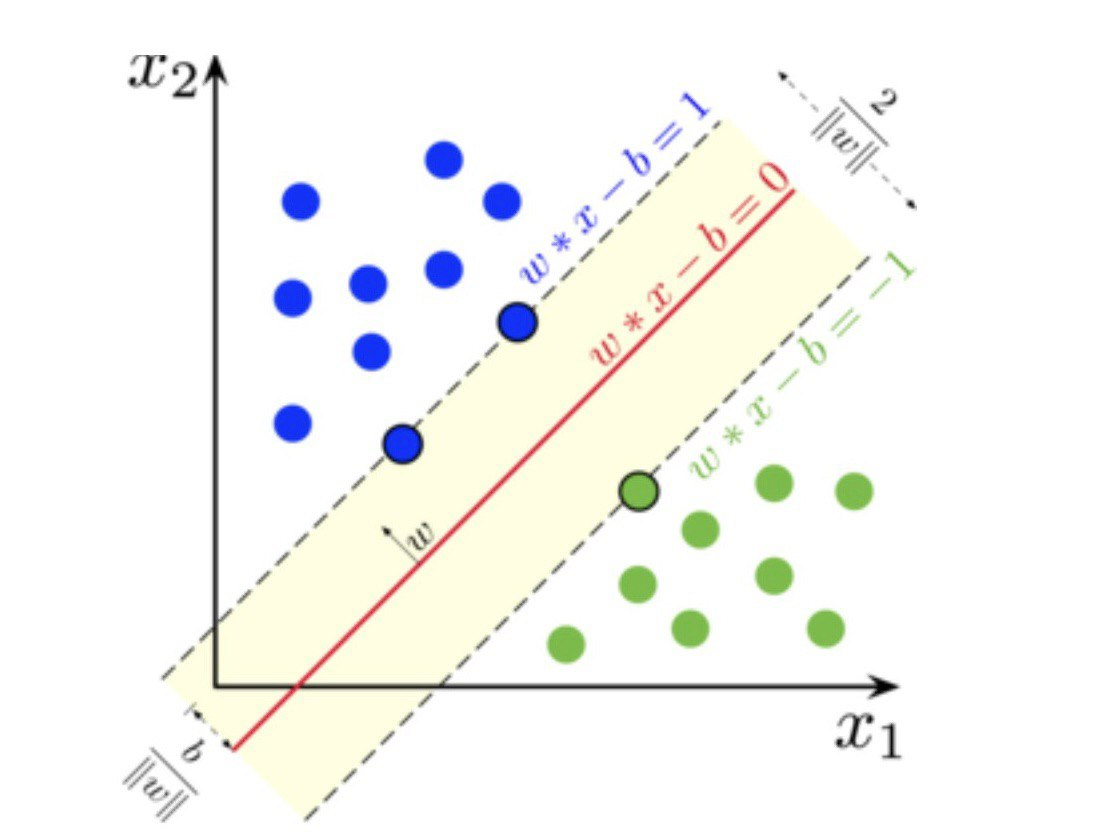
\includegraphics[width=0.75\linewidth]{images/SVM_margin.jpg}
    \caption{Machines à vecteur de support pour une classification binaire}
    \label{fig:fig11}
\end{figure}

\subsection{Les machines à vecteur de support pour la détection d'anomalie}
\label{chap4.sec8.sub1}
Un détail que je n'ai pas précisé avec les autres modèles est que l'ensemble de données que j'avais à disposition pour ce travail était très déséquilibré. Sur les 1.526.659 exemples il n'y avait que 47.994 qui avait faillit sur leur prêt, soit approximativement 3\% de l'ensemble de données. C'est une situation qui peut arriver dans certaines applications où les différentes classes sont naturellement déséquilibrés, la section \ref{chap4.section9} sera dédiée à expliquer ce problème et les solutions que j'ai mis en place pour essayer de minimiser l'impact sur les modèles de classification.

Cette section n'était pas censé faire partie du document initialement, tout vient de l'idée qu'avec un ensemble de données si déséquilibré, un modèle de detection d'anomalies\footnote{La détection d'anomalies est un domaine essentiel de l'analyse de données et de l'apprentissage automatique, qui consiste à identifier des observations ou des événements rares et atypiques dans un ensemble de données. Ces anomalies peuvent indiquer des erreurs, des fraudes, des pannes ou d'autres phénomènes inhabituels qui nécessitent une attention particulière.} pourrait s'averer meilleur pour distinguer les deux classes. Donc l'idée m'a été proposer d'implémenter un modèle de detection d'anomalies qui sera utiliser comme un modèle de classification dans le soucis de déterminer correctement les clients qui sont plus susceptibles de faire défaut sur leur prêt.

Dans un papier de 1999, Bernhard Scholkopf et al ont proposé un algorithme de machine à vecteur de support pour aborder le problème de détection d'anomalies en essayant d'estimer un
fonction \(f\) qui est positive sur un sous-ensemble \(S\) des données (considéré comme normal) et négative sur le complément (considéré comme anomalie). Leur méthode est un algorithme d'apprentissage non supervisé qui prend un ensemble de données \(X\) le projette dans un espace dimensionnel plus grand et cherche les paramètres de l'hyperplan qui englobe la majeur partie des données tout en maximisant la marge entre les points de données et l'origine de l'espace dimensionnel (\cite{scholkopf1999support}). Le resultat est un modèle qui, une fois entraîné, évalue si un nouveau point de donnée tombe dans cet hyperplan (normal) ou à l'extérieur (anomalie).

\subsection{Impémentation}
\label{chap4.sec8.sub2}
J'ai donc testé cet algorithme, en entraînant un modèle sur un sous-ensemble des clients qui avait remboursé leurs prêts (un peu à la dernière minute), ce qui a justifié l'ajout de cette section. L'implémentation est basé sur celle de scikit-learn de l'algorithme de Scholkopf et al. Par contre l'algorithme est très inefficace en termes de temps ce qui m'a obligé à entraîner seulement sur 100.000 exemples (\cite{diarra2024anomaly}).